\documentclass{amsart}
\usepackage{hyperref}
\usepackage{fullpage}
\usepackage{amsrefs}
\usepackage{verbatim}
\usepackage{tikz}
\usetikzlibrary{matrix,arrows,decorations.pathmorphing, cd}

\newcommand{\Map}       {\operatorname{Map}}

\newcommand{\sgn}	{\operatorname{sgn}}
\newcommand{\lnk}	{\operatorname{link}}

\newcommand{\N}         {{\mathbb{N}}}
\newcommand{\Z}         {{\mathbb{Z}}}
\newcommand{\R}         {{\mathbb{R}}}

\newcommand{\al}        {\alpha}
\newcommand{\bt}        {\beta} 
\newcommand{\gm}        {\gamma}
\newcommand{\dl}        {\delta}
\newcommand{\zt}        {\zeta}
\newcommand{\tht}       {\theta}
\newcommand{\lm}        {\lambda}
\newcommand{\sg}        {\sigma}

\newcommand{\Dl}        {\Delta}
\newcommand{\Lm}        {\Lambda}

\newcommand{\ho}	{\widehat{o}}
\newcommand{\hp}	{\widehat{p}}
\newcommand{\hpi}	{\widehat{\pi}}

\newcommand{\fr}[4]{\fill (#1,#2) rectangle (#3,#4);}
\newcommand{\fg}[4]{\fill[gray] (#1,#2) rectangle (#3,#4);}
\newcommand{\gr}[1]{\foreach \i in {0,1,...,#1} {\draw(\i,0) -- (\i,#1); \draw(0,\i) -- (#1,\i);}}

\newcommand{\xra}       {\xrightarrow}
\newcommand{\sm}        {\setminus}
\newcommand{\st}        {\;|\;}
\newcommand{\sse}       {\subseteq}
\newcommand{\tm}        {\times}
\newcommand{\bbm}       {\left[\begin{matrix}}
\newcommand{\ebm}       {\end{matrix}\right]}


\renewcommand{\:}{\colon}

\newtheorem{theorem}{Theorem}[section]
\newtheorem{conjecture}[theorem]{Conjecture}
\newtheorem{lemma}[theorem]{Lemma}
\newtheorem{proposition}[theorem]{Proposition}
\newtheorem{corollary}[theorem]{Corollary}
\theoremstyle{definition}
\newtheorem{remark}[theorem]{Remark}
\newtheorem{definition}[theorem]{Definition}
\newtheorem{example}[theorem]{Example}
\newtheorem{construction}[theorem]{Construction}

\newtheorem{notation}{Notation}
\renewcommand{\thenotation}{} % make the notation environment unnumbered

%\numberwithin{equation}{subsection}

\begin{document}
\title{Small exact neural networks}
\author{N.~P.~Strickland}

\maketitle 


Here we discuss some neural networks where one can specify the weights
explicitly. 

\section{Binary boolean functions}

We can represent truth values by $0$ and $1$.  There are $16$
possible boolean functions of two arguments, and they can all be
represented by $2$-layer networks.  Explicitly, if $x,y\in\{0,1\}$
then $xy=(x+y-1)_+$.  Now suppose we have $f\:\{0,1\}^2\to\R^m$ with 
\[ f(0,0) = u_0 \qquad f(0,1) = u_1 \qquad 
   f(1,0) = u_2 \qquad f(1,1) = u_3.
\]
We then find that 
\[ f(x,y) = u_0 + (u_2-u_0)x + (u_1-u_0)y + (u_3-u_2-u_1+u_0)xy. \]
This leads to an evident encoding of $f$ as a RELU layer (encoding
$(x,y)\mapsto(x,y,xy)$) followed by a linear layer.  In particular, we
can apply this to the function $f\:\{0,1\}^2\to\R^{16}$ which computes
all $16$ boolean functions simultaneously.  This is implemented in the
file \texttt{bool.py}.

A similar construction computes any function of $n$ boolean variables
as a RELU layer with $2^n-1$ outputs followed by a linear layer.  For
particular boolean functions it will be more efficient to use a deeper
network.  

\section{Digit recognition}

A standard initial exercise in Machine Learning is to recognise
images of handwritten digits from the mnist dataset.  Here we do an
even simpler version of that.

Consider digits drawn as $6\tm 6$ pixel images using straight
horizontal and vertical lines, as illustrated below.
\begin{center}
 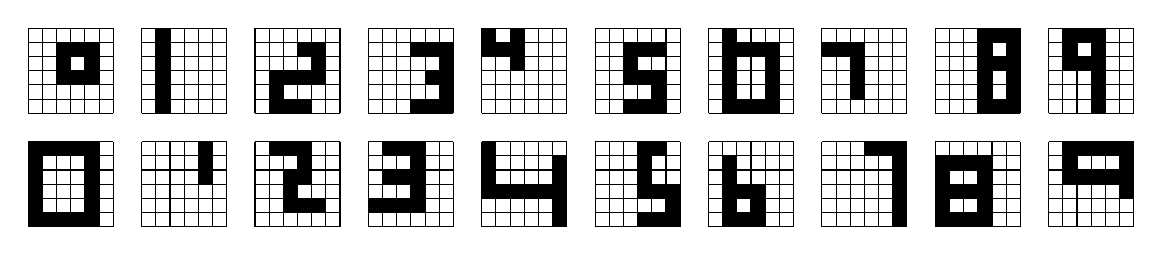
\begin{tikzpicture}[scale=0.18]
  \begin{scope}[shift={( 0, 0)}] \gr{6} \fr0041\fr0546\fr0015\fr4056 \end{scope}
  \begin{scope}[shift={( 8, 0)}] \gr{6} \fr4356 \end{scope}
  \begin{scope}[shift={(16, 0)}] \gr{6} \fr2152\fr2234\fr3346\fr1536 \end{scope}
  \begin{scope}[shift={(24, 0)}] \gr{6} \fr0142\fr3246\fr1334\fr1536 \end{scope}
  \begin{scope}[shift={(32, 0)}] \gr{6} \fr0253\fr0316\fr5065 \end{scope}
  \begin{scope}[shift={(40, 0)}] \gr{6} \fr3061\fr5163\fr3253\fr3346\fr4556 \end{scope}
  \begin{scope}[shift={(48, 0)}] \gr{6} \fr1041\fr1125\fr2243\fr3142 \end{scope}
  \begin{scope}[shift={(56, 0)}] \gr{6} \fr5066\fr3556 \end{scope}
  \begin{scope}[shift={(64, 0)}] \gr{6} \fr0041\fr0243\fr0445\fr0015\fr3045 \end{scope}
  \begin{scope}[shift={(72, 0)}] \gr{6} \fr1364\fr1566\fr1425\fr5266 \end{scope}
  \begin{scope}[shift={( 0, 8)}] \gr{6} \fr2253\fr2455\fr2334\fr4354 \end{scope}
  \begin{scope}[shift={( 8, 8)}] \gr{6} \fr1026 \end{scope}
  \begin{scope}[shift={(16, 8)}] \gr{6} \fr1041\fr1123\fr2253\fr4355\fr3445 \end{scope}
  \begin{scope}[shift={(24, 8)}] \gr{6} \fr3061\fr4263\fr3465\fr5065 \end{scope}
  \begin{scope}[shift={(32, 8)}] \gr{6} \fr0416\fr1425\fr2336 \end{scope}
  \begin{scope}[shift={(40, 8)}] \gr{6} \fr2051\fr4153\fr2243\fr2335\fr3455 \end{scope}
  \begin{scope}[shift={(48, 8)}] \gr{6} \fr1051\fr1455\fr1026\fr4055 \end{scope}
  \begin{scope}[shift={(56, 8)}] \gr{6} \fr0435\fr2134 \end{scope}
  \begin{scope}[shift={(64, 8)}] \gr{6} \fr3061\fr3364\fr3566\fr3046\fr5066 \end{scope}
  \begin{scope}[shift={(72, 8)}] \gr{6} \fr1334\fr1536\fr1425\fr3046 \end{scope}
 \end{tikzpicture}
\end{center}
We can build a neural network to recognise such digits as described
below.  The first step is a convolutional layer with twelve kernels of
shape $3\tm 3$, whose effect is illustrated by the pictures below.
\begin{center}
 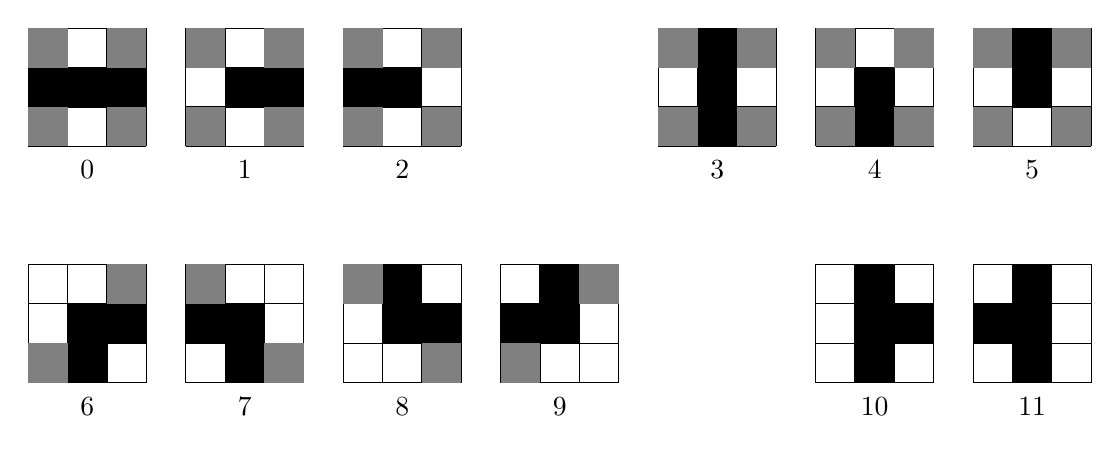
\begin{tikzpicture}[scale=0.5]
  \begin{scope}[shift={( 0, 6)}] \gr{3} \fr0132\fg0011\fg0213\fg2233\fg2031 \draw(1.5,-0.6) node{$ 0$}; \end{scope}
  \begin{scope}[shift={( 4, 6)}] \gr{3} \fr1132\fg0011\fg0213\fg2233\fg2031 \draw(1.5,-0.6) node{$ 1$}; \end{scope}
  \begin{scope}[shift={( 8, 6)}] \gr{3} \fr0122\fg0011\fg0213\fg2233\fg2031 \draw(1.5,-0.6) node{$ 2$}; \end{scope}
  \begin{scope}[shift={(16, 6)}] \gr{3} \fr1023\fg0011\fg2031\fg2233\fg0213 \draw(1.5,-0.6) node{$ 3$}; \end{scope}
  \begin{scope}[shift={(20, 6)}] \gr{3} \fr1022\fg0011\fg2031\fg2233\fg0213 \draw(1.5,-0.6) node{$ 4$}; \end{scope}
  \begin{scope}[shift={(24, 6)}] \gr{3} \fr1123\fg0011\fg2031\fg2233\fg0213 \draw(1.5,-0.6) node{$ 5$}; \end{scope}
  \begin{scope}[shift={( 0, 0)}] \gr{3} \fr1022\fr2132\fg0011\fg2233        \draw(1.5,-0.6) node{$ 6$}; \end{scope}
  \begin{scope}[shift={( 4, 0)}] \gr{3} \fr1022\fr0112\fg0213\fg2031        \draw(1.5,-0.6) node{$ 7$}; \end{scope}
  \begin{scope}[shift={( 8, 0)}] \gr{3} \fr1123\fr2132\fg0213\fg2031        \draw(1.5,-0.6) node{$ 8$}; \end{scope}
  \begin{scope}[shift={(12, 0)}] \gr{3} \fr0122\fr1223\fg0011\fg2233        \draw(1.5,-0.6) node{$ 9$}; \end{scope}
  \begin{scope}[shift={(20, 0)}] \gr{3} \fr1023\fr2132                      \draw(1.5,-0.6) node{$10$}; \end{scope}
  \begin{scope}[shift={(24, 0)}] \gr{3} \fr1023\fr0112                      \draw(1.5,-0.6) node{$11$}; \end{scope}
 \end{tikzpicture}
\end{center}
In more detail, we say that a pixel has type $i$ if the surrounding
$3\tm 3$ block matches the above picture marked $i$, in the sense
that black pixels must be black, white pixels must be white, and grey
pixels can be either colour.  To interpret this for pixels on the
edge, we assume that the image is surrounded by white pixels.  For a
valid digit image, each black pixel must have type $i$ for some $i$.
If we start with an image represented as an element of
$M_6(\{0,1\})$, then the convolutional layer will replace it by an
element of $M_6(\{0,1\}^{12})$.  If a pixel has type $i$ for some
$i$, then the corresponding entry in the new matrix will be $e_i$.
If a pixel does not have type $i$ for any $i$ then the corresponding
entry will be $0$.  

We can now take the sum over all matrix entries to count the total
number of pixels of each type.  The numbers for types $0$ and $3$
will depend on the precise geometry of the represented digit, but the
numbers for the other types will not.  These numbers are sufficient
to distinguish all digits except for $2$ and $5$.  To distinguish
these, we need to check whether the pixels of types $6$ and $8$
appear above or below those of types $7$ and $9$, which is also
easily done by a neural network layer.  All this is implemented in
\texttt{digits.py}.  The method used there does not always
reject non-digits; ideally it should be enhanced to do that.

We have also trained a neural network in the conventional way to
perform the same task.  We can achieve perfect performance with a
smaller model than the handcrafted model described above.
Specifically, we have a model consisting of a $3$-channel
convolutional layer with kernels of size $3\times 3$, followed by a
dense layer with $3$ outputs, followed by a dense layer with $10$
outputs.  We train this model to predict the one-hot encoding of the
relevant digit, and then apply argmax to predict the digit itself.

For the convolutional layer, we can interpret the three output
channels as red, green and blue, so the layer has the effect of
colouring the image.  The kernels can be displayed as follows:
\begin{center}
 \includegraphics[scale=0.5]{digit_kernels.png}
\end{center}

The effect on a random selection of examples is shown below.
\begin{center}
 \includegraphics[scale=0.5]{digit_features.png}
\end{center}

The output of the second layer gives a point in $\R^3$ for each digit
image.  These points are best displayed using a 3D viewer which allows
the diagram to be rotated interactively.  The figure below shows the
view from one angle (with different digits marked in different colours).
\begin{center}
 \includegraphics[scale=0.5]{digit_embedding.png}
\end{center}

\section{Noughts and crosses}

We would like to train a neural network to play noughts and crosses
(also known as Tick Tack Toe).  Code for this is in the file
\texttt{ox.py} (and also the Maple worksheet \texttt{ox.mw}). 

The game is played on a $3\tm 3$ board; we number the board positions
as $0,\dotsc,8$ in the obvious way.  We have two players: player $0$
places Os on the board and player $1$ places Xs on the board.  We
represent the game state as an array of shape $9\tm 2$, with a $1$ at
position $(i,j)$ if player $j$ has placed a counter at position $i$.
There are $8$ horizontal, vertical or diagonal lines on the board,
corresponding to the following sets of positions:
\[ W = \{\{0,3,6\}, \{1,4,7\}, \{2,5,8\}, 
         \{0,1,2\}, \{3,4,5\}, \{6,7,8\},
         \{0,4,8\}, \{2,4,6\}\}.
\]
A player wins if they have covered at least one of these lines.

We are mostly interested in game states such that
\begin{itemize}
 \item[(a)] The state is empty or could be reached by a legal sequence
  of moves with the last move played by player 1.
 \item[(b)] The game has not finished, so neither player has won, and
  there is at least one blank spot on the board.
\end{itemize}
Let $X$ be the set of states of this type.  We find that $|X|=4519$.
We want a function $F$ that accepts an element of $X$ and generates a
probability distribution on the board positions.  Player $0$ can then
sample randomly from that distribution to decide where to play.  This
may result in an illegal move, where the selected position is already
occupied; if so we declare that player $0$ has lost.

There is a well-known function $F_1$ which is optimal: if a player
uses that algorithm then they are guaranteed to win or draw.

The most obvious approach is just to train a model to replicate the
behaviour of $F_1$.  We have successfully done this, with two hidden
layers of size $20$ between the input layer (of shape $9\times 2$) and
the output layer (of size $9$).

We have also attempted to do two different flavours of reinforcement
learning: a policy gradient approach and a deep Q-learning approach.
Neither has so far been successful.  It is not clear whether our
implementation is flawed or whether our training hyperparameters are
inappropriate.

\section{Conway's Game of Life}

Conway's Game of Life can be described as follows.  Fix $N$ and let
$X$ be the set of $N\tm N$ matrices with entries in $\{0,1\}$.  For
$A\in X$ we have $A_{ij}\in\{0,1\}$ for $0\leq i,j<N$, and we take
$A_{ij}$ to be $0$ for all other pairs $(i,j)$.  In this extended
matrix, every entry $A_{ij}$ has $8$ adjacent entries; we define
$(NA)_{ij}$ to be the sum of these.  We then define $(PA)_{ij}$ to be
$1$ if $0\leq i,j<N$ and (($A_{ij}=0$ and $(NA)_{ij}=3$) or  
($A_{ij}=1$ and $(NA)_{ij}\in\{2,3\}$)).  This defines $P\:X\to X$,
and the idea is to study the sequence $(P^nA)_{n\in\N}$.  Here,
however, we just want a convolutional neural network to calculate the
function $P$.  The first step is to define $QA=A+2NA$; we then have
$(PA)_{ij}=1$ iff $(QA)_{ij}\in\{5,6,7\}$.  Also, if we put 
\[ f(x)=(x-4)_+ - (x-5)_+ - (x-7)_+ + (x-8)_+,\]
we find that for $x\in\Z$ we have $f(x)=1$ if $x\in\{5,6,7\}$ and
$f(x)=0$ otherwise; so $(PA)_{ij}=f((QA)_{ij})$.  This description of
$P$ can be translated in a straightforward way into a convolutional
neural network, as is done in the file \texttt{life.py}.

\section{Resettable running total}

\begin{example}\label{eg-running}
 Given an infinite sequence of natural numbers $(x_i)_{i\geq 0}$, we
 can define $y_0=x_0$ and 
 \[ y_{i+1} = \begin{cases}
     y_i+x_{i+1} & \text{ if } x_{i+1} > 0 \\
     0 & \text{ if } x_{i+1} = 0.
    \end{cases}
 \]
 In other words, our output is the running total of the inputs, except
 that the total resets to zero whenever the input is zero.  This can
 be computed by a Gated Recurrent Unit network (GRU), as is done in
 \texttt{rnn.py}. 
\end{example}

\section{Miscellaneous other examples}

\begin{example}\label{eg-intervals}
 For integer $x$ we find that  
 \begin{align*}
  (n-x)_+ - (n-1-x)_+ &= I(x\geq n) \\
  1 - (n-x)_+ + (n-1-x)_+ &= I(x < n) \\
  (n+1-x)_+ - 2(n-x)_+ + (n-1-x)_+ &= I(x = n).
 \end{align*}
 It follows that these functions can be computed by $2$-layer networks
 with RELU activation in the first layer.  The same therefore holds
 for composites of these functions with additive functions
 $\Z^n\to\Z$.

 It seems that standard training algorithms struggle to find these
 weights. 
\end{example}

\begin{example}\label{eg-first}
 Given a list $(x_0,\dotsc,x_{n-1})\in\{0,1\}^n$, we can define
 $y_i=p\left(x_i-\sum_{j<i}x_j\right)$.  If $x=0$ then $y=0$.
 Otherwise, if $i$ is least such that $x_i=1$ then $y=e_i$.
\end{example}

\begin{example}\label{eg-delta}
 Suppose that $u\in\{0,1\}^n$, and define $f\:\{0,1\}^n\to\{0,1\}$ to
 be the delta function concentrated at $u$.  Put $U=\{i\st u_i=1\}$
 and $e=(1,\dotsc,1)\in\{0,1\}^n$.  We then find that 
 \begin{align*}
  f(x) &=
   \left(1+\sum_{i\in U}(x_i-1)-\sum_{i\not\in U}x_i\right)_+  \\
  &= \left(1 + (x - e).u - (e-u).x\right)_+ 
   = \left(1-e.u+(2u-e).x\right)_+.
 \end{align*}
 Thus, $f$ can be calculated by a one-layer RELU network.  This is
 used as an ingredient in many of the examples described later.

 Suppose we wanted to train a network to calculate $f$.  If we work in
 terms of the variables $2x_i-1\in\{1,-1\}$ then a change in $u$ just
 corresponds to multiplying some weights by $-1$.  Thus, we can
 restrict attention to the case $u=e$, where $f(x)=(e.x-(n-1))_+$.  

 Put $X=\{x\in\{0,1\}^{n+1}\st x_0=1\}$ and $e'=(1,\dotsc,1)\in X$.
 We want to find $a\in\R^{n+1}$ such that $(a.x)_+=\dl_{x,e'}$ for all
 $x\in X$, so we use the loss function 
 \[ L(a) = \sum_{x\in X}((a.x)_+-\dl_{x,e'})^2/2. \]
 Note that there are actually many solutions $a$ with $L(a)=0$: they
 are given by $a_0=1-\sum_{i=1}^na_i$ with $a_i\geq 1$ for
 $i=1,\dotsc,n$.  Any reasonable regularisation penalty should pick
 out the solution where $a_0=1-n$ and $a_i=1$ for $i>0$.

 Put $X_i=\{x\in X\st x_i=1\}$.  We find that the partial derivatives
 are 
 \[ L_{,i}(a) = \sum_{x\in X_i}(a.x)_+ - H(a.e'), \]
 where $H$ is the Heaviside function.  When $a$ is close to a solution
 then the terms $(a.x)_+$ will be small for $x\in X_i\sm\{e'\}$, and
 $H(a.e')$ will be $1$, and $(a.e')_+-1$ will also be small, so
 $L_{,i}(a)$ will be small.  There is code for this analysis in
 \texttt{maple/train\_delta.mw}. 
\end{example}

\begin{example}\label{eg-binary-words}
 It should be possible to write an explicit network to translate
 English to German, where the only allowed English words are ``zero''
 and ``one'' (to be translated as ``null'' and ``eins'').  Text
 processing networks typically start with a word tokenizer, which
 would make the problem trivial.  Instead we should assume that the
 input is given as a sequence of characters.
\end{example}

\begin{example}\label{eg-letters}
 The letters C,H,I,J,L,O,T,U,X,Y can be represented using as $3\times 3$
 pixel images.  These are shown below, grouped according to the number of 
 black pixels. 
 \begin{center}
  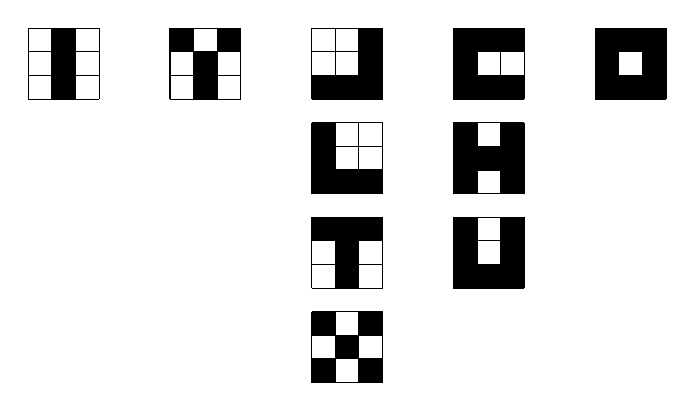
\begin{tikzpicture}[scale=0.3]
   \begin{scope}[shift={( 0,  0)}] \gr{3} \fr1023                      \end{scope} % I
   \begin{scope}[shift={( 6,  0)}] \gr{3} \fr1022\fr0213\fr2233        \end{scope} % Y
   \begin{scope}[shift={(12,  0)}] \gr{3} \fr0031\fr2133               \end{scope} % J
   \begin{scope}[shift={(12,- 4)}] \gr{3} \fr0031\fr0113               \end{scope} % L
   \begin{scope}[shift={(12,- 8)}] \gr{3} \fr1022\fr0233               \end{scope} % T
   \begin{scope}[shift={(12,-12)}] \gr{3} \fr0011\fr2031\fr1122\fr0213\fr2233 \end{scope} % X
   \begin{scope}[shift={(18,  0)}] \gr{3} \fr0031\fr0112\fr0233        \end{scope} % C
   \begin{scope}[shift={(18,- 4)}] \gr{3} \fr0013\fr1122\fr2033        \end{scope} % H
   \begin{scope}[shift={(18,- 8)}] \gr{3} \fr0013\fr1021\fr2033        \end{scope} % U
   \begin{scope}[shift={(24,  0)}] \gr{3} \fr0031\fr0112\fr2132\fr0233 \end{scope} % O
  \end{tikzpicture}
 \end{center}
 It should be possible to write an explicit network to
 recognise them, and then make a convolutional version to find them in
 a larger grid.  Then we could perhaps try to count the number of
 appearances of each letter.  The file \verb+words_3x3.txt+ contains 
 181 words that use only the letters listed here; we could also try to
 detect and count these words.
\end{example}

\begin{example}\label{eg-pl}
 Consider a piecewise-linear function $f\:\R\to\R$ with finitely many
 corners, so there are real numbers $a_1<\dotsb<a_r$ and slopes
 $m_0,\dotsc,m_r$ and a constant $c$ such that 
 \begin{itemize}
  \item[(a)] $f(x)=m_0x+c$ on $(-\infty,a_1]$
  \item[(b)] $f(x)$ has slope $m_i$ on $[a_i,a_{i+1}]$ for
   $i=1,\dotsc,r-1$
  \item[(c)] $f(x)$ has slope $m_r$ on $[a_r,\infty)$.
 \end{itemize}
 Then 
 \[ f(x) = c + m_0 x + \sum_{i=1}^r (m_i-m_{i-1})(x-a_i)_+. \]
 However, the situation with piecewise-linear functions in more than
 one variable seems unclear.
\end{example}




\end{document}
